Proteins are key actors of biological processes inside cells. Rather
than carrying out tasks as single agents, they are part of dynamic
networks of protein-protein interactions (PPI) \cite{Lin2017}. Such
networks underlie a variety of interdependent mechanisms, including
signal transduction, homeostasis control and stress responses. Furthermore,
PPI networks play an important role in physiological and developmental
processes such as protein phosphorylation, transcriptional co-factor
recruitment and transporter activation \cite{Zhang2010PPI}.

A common way to create PPI networks (or validate particular protein-protein
interactions) is the \emph{Yeast-Two-Hybrid} technique (also known
as \emph{two-hybrid screening} or \emph{Y2H}). Figure \ref{Y2H}A
illustrates the biological basis of Y2H: the expression of a specific
reporter gene is activated by the binding of a DNA-binding Domain
(DB) and an Activation Domain (AD) of a Transcription Factor, which
in turn binds to an Upstream Activation Sequence (UAS). To evaluate
an interaction between two proteins, the Y2H approach fuses one protein
to the DB domain (known as \emph{bait}) and the other to the
AD (known as \emph{prey}). If the proteins interact, the reporter
gene expression is activated by the AD (Fig. \ref{Y2H}B). Otherwise,
if proteins fail to interact, the reporter gene is not expressed (Fig.
\ref{Y2H}C).

\begin{figure}[h]
\caption{\label{Y2H}The Yeast-2-Hybrid technique offers an experimental approach
for constructing PPI networks.}
\centering
	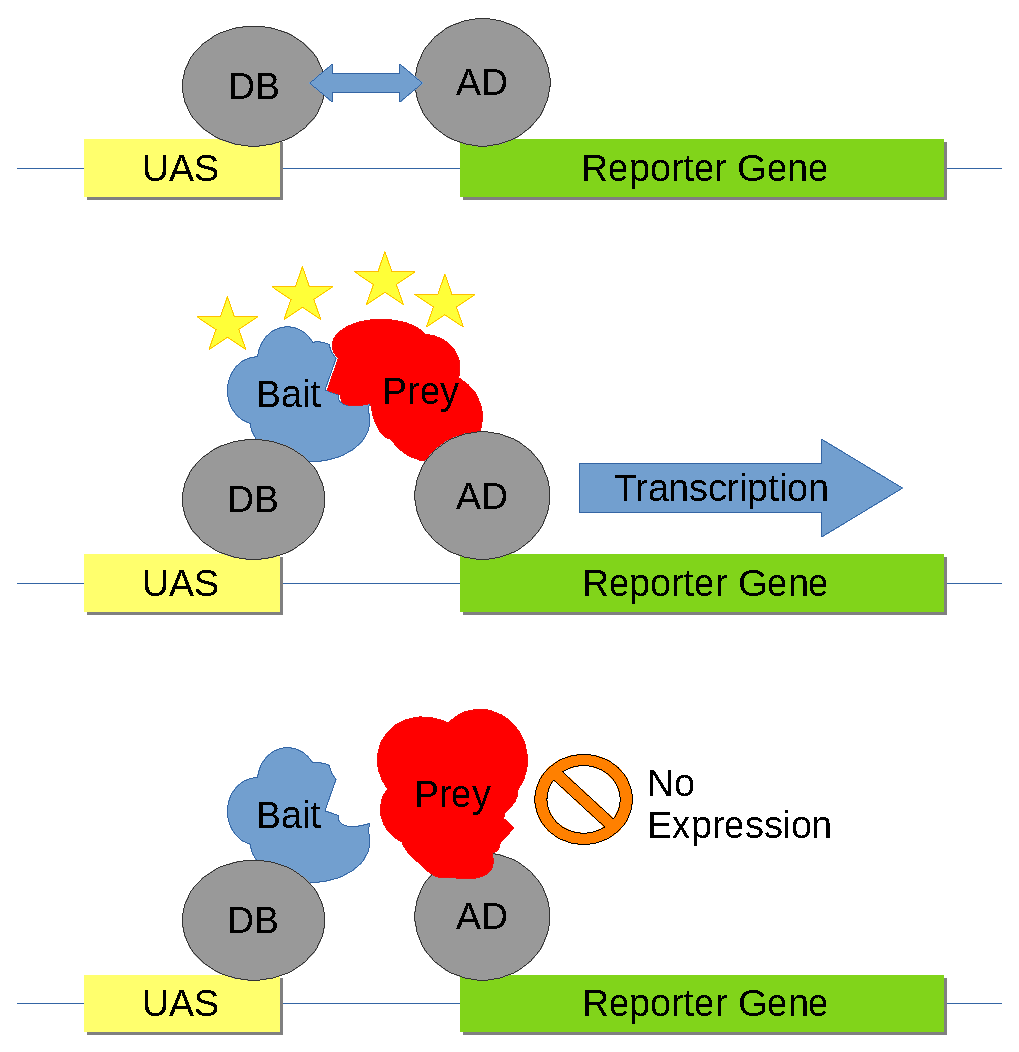
\includegraphics[width=0.7\columnwidth]{../Y2H}
\end{figure}

Based on the outcome of Y2H experiments, numerous networks
of interactions between proteins have been constructed \cite{Weimann2013Y2H,Rajagopala2015Y2H,Shokri2019TFY2H}.
However, identifying protein interactions through Y2H experiments is costly in terms of time
and resources\cite{Laraia2015PPI,Macalino2018PPI}. For an organism with 2000
unique proteins, for example, a detailed PPI network requires the experimental
validation of around 2 million interactions. The number of missing
interactions for pairs of proteins on many organisms require the
use of computational tools for predicting such interactions.

Different methods for predicting interactions in PPI networks have
been proposed \cite{Chang2016PPI,Chen2019PPI,Kotlyar2015PPI}. A 
common approach for predicting PPIs is based the triadic closure principle
(TCP). TCP states that the higher the number of common neighboring
nodes between two nodes, the higher the probability that they interact
\cite{Goldberg2003SmallWorld}. TCP can be addressed mathematically
by counting the number of shared neighbors of a pair of nodes, also
known as the Common Neighbors algorithm. By raising the adjacency
matrix (A) of the PPI network to the second power (A\texttwosuperior ),
the provides an insight into which proteins may interact with each other. However, previous studies
show that this mentioned approach alone usually fails because it does not
consider the structural and chemical properties of the proteins \cite{Cannistraci2013Networks,Kovacs2019}.

Kovacs et al (2019) introduce a network-based approach which predicts
an interaction between two proteins based on the number of paths
of length 3. The number of paths of length 3 is computed by raising
the adjacency matrix of the network to the third power (A\textthreesuperior).
The degree-normalized measure, denoted as L3,  mitigates bias caused by
intermediate hubs within the paths of length 3. The measure L3 enables
the approach in Kovacs et al (2019) to outperform previous methods for predicting
binary protein interactions for various organisms, including yeast (\emph{S. cerevisiae}),
Arabidopsis (\emph{A. thaliana}), worm (\emph{C. elegans}), fly (\emph{D. melanogaster}),
fission yeast (\emph{S. pombe}), mouse (\emph{M. musculus}) and humans
\cite{Kovacs2019}.

Our work extends previous analyses by using handcrafted features (A2,
A3, L3) as well as a low-dimensional representation of nodes 
(\texttt{Node2Vec})\cite{Grover_2016} for PPI networks in the human and rice 
interactomes. To evaluate the proposed approach, we try to predict interactions
using a state-of-the-art Machine Learning algorithm called \texttt{XGBoost}\cite{2016ChenXGB},
which uses a gradient boosted decision tree model to weigh the features.
Our main results show that adding the handcrafted features derived from the
network connectivity to the Machine Learning model improve the prediction
power of the models. This property can be assessed when looking at the their
importance in the model.  The main contributions of this paper are i) a
general framework for link prediction in non-directed networks and ii) two
applications of this framework to biological networks with a structural
insight.

\paragraph*{Document structure:} This paper is organized as follows. \emph{Materials and Methods} describes
the methodological steps and key milestones in the preparation of
the networks, model parameters and experimental configurations.
\emph{Results} presents the main results of the models for the human and rice interactomes.
\emph{Conclusions} presents the main conclusions of this study. Finally, the \emph{appendix}
presents supplementary information and figures which complement the
results described in this paper.